\documentclass{report}
\usepackage{polyglossia}
\usepackage{graphicx}
\usepackage{fixlatvian}
\usepackage{verbatim}
\usepackage{pgfplots}
\usepackage{circuitikz}


\title{Report on Labratory work 1}
\author{Grats Grāvelsins}
\date{March 2018}

\begin{document}
\maketitle

\chapter{Teorētiska daļa}

\section{Ķēdes aprēķins}
Sprieguma avota V1 sprieguma vērtību U-(Voltos) izvēlējos daļskaitli, kas is manas apliecības pēdējie trīs cipari dalīti ar 10. Piemēram.
171REB073 nozīmē V1 = 7.3 (Volti), R1 ir apliecības pēdējo 3 ciparu otrais numurs+1, R2 ir apliecības numura pēdējais cipars +1. Piemēram, ja Jūsu apliecības numurs ir 171REB073, tad R1=8,R2=4


\begin{table}
\begin{tabular}{|c|c|}
\hline
R1 & 8 \\
\hline
R2 & 4 \\
\hline
V1 & 7.3  \\
\hline 
UR2 & 5.2 \\
\hline
UR1 &  6.3 \\
\hline
\end{tabular}
\begin{centering}
\caption{Sprieguma un prestestības tabula}
\end{centering}
\end{table}

\begin{figure}
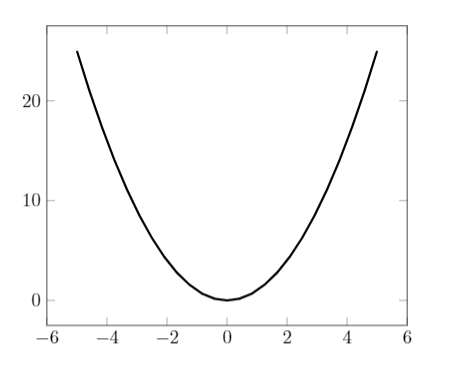
\includegraphics[width=8cm]{grafiks.png}
\caption{Sprieguma grafiks}
\end{figure}

\begin{center}
\begin{circuitikz}[american voltages]
\draw
(0,4) to [V, l_=$Us$] (0,0)
to [short, *-] (6,0)
to (6,2)
to [R, l_=$R$] (6,4)
to [short, ] (5,4)
to (3,4) to [open, ] (0,4)
to [short, ] (1,4)
to [R, l=$R$] (3,4)
to (4,4)
;
\end{circuitikz}
\end{center}




\chapter{Praktiskā daļa}
\section{Darbs ar GEDA programmām}
\subsection{Darbs ar gschem}

\begin{figure}[h]
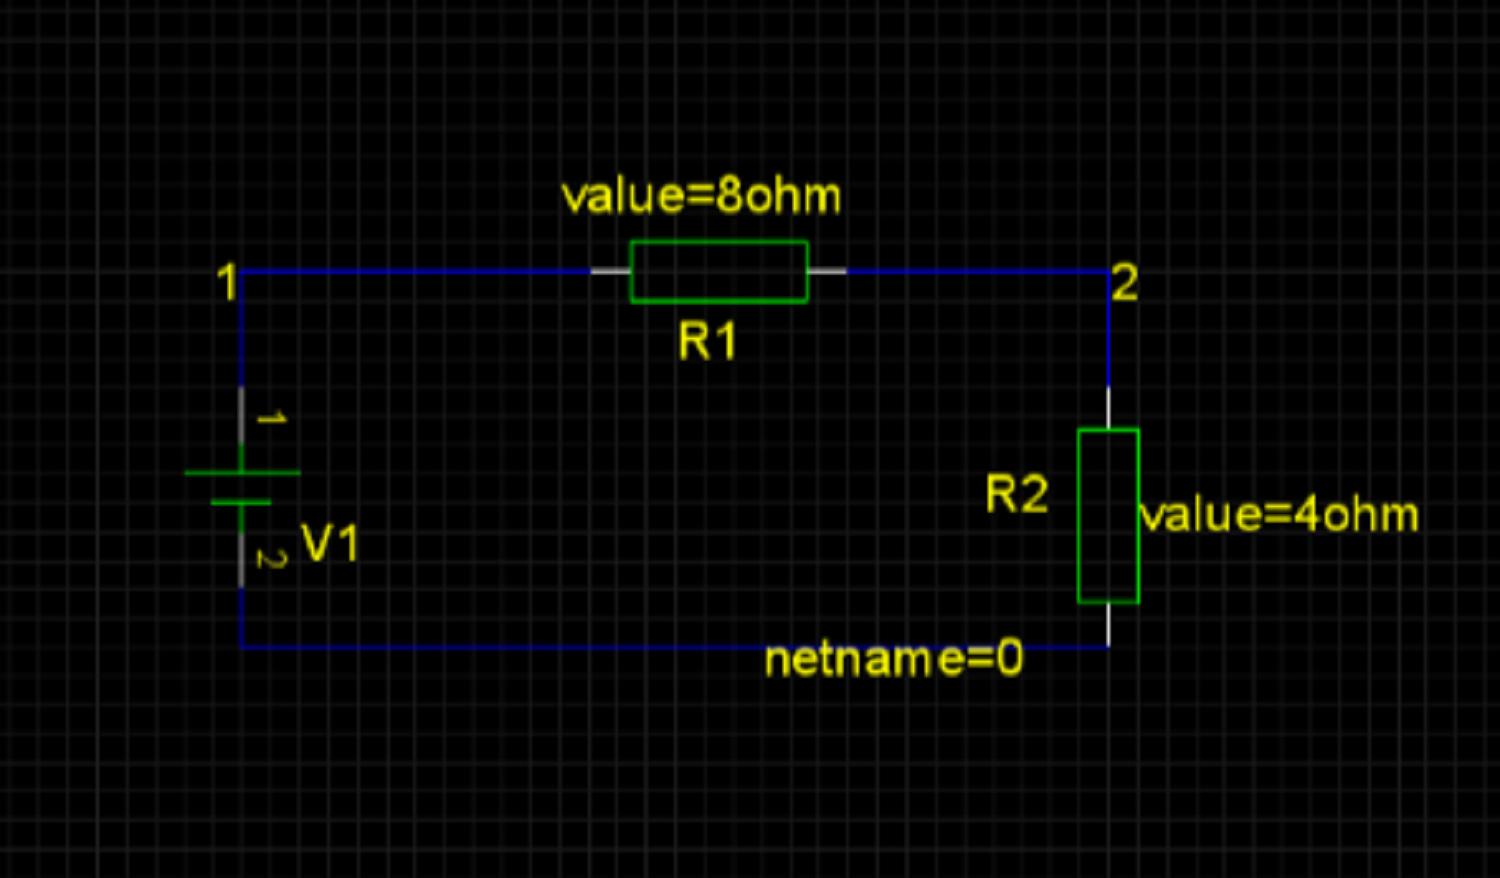
\includegraphics[width=\textwidth]{shnr1.png}
\caption{Elektriskā shēma}
\label{2}
\end{figure}
\newpage
\subsection{Darbs ar gnetlist}
\verbatiminput{01.net}

\subsection{Darbs ar ngspice}
\begin{figure}[h]
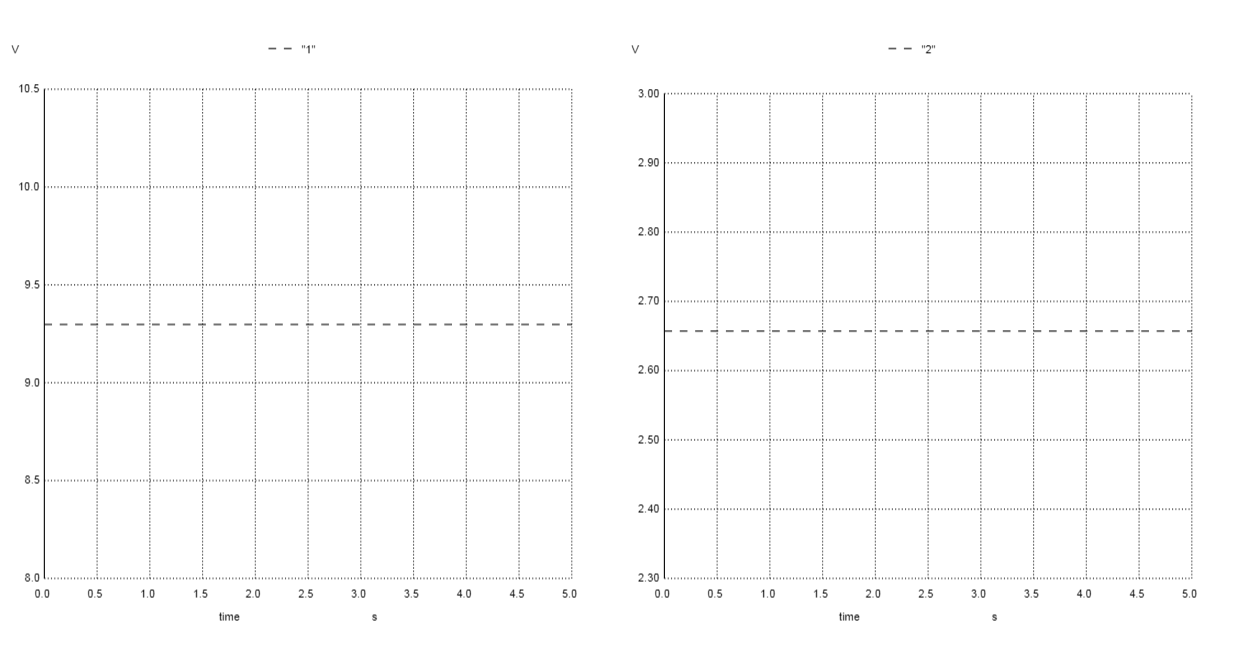
\includegraphics[width=\textwidth]{divigraf.png}
\caption{NGspice iegūtais grafiks}
\vspace{10mm}
Grafiki tiki novietoti blakus, lai labāk pārskatāmi!
\label{fig:011.ps}

\end{figure}



\section{Darbs ar QUCS programmām}
\rotatebox{-90}{\includegraphics[width=30cm]{s1.ps}}
\subsection{Tabula un grafiki}
\rotatebox{-90}{\includegraphics[width=20cm]{tabula01.ps}}
\subsection{Secinājumi}
1. Parameter sweep palīdz attēloot visu nepieciešamo informāciju
saslēgtajai ķēdei, šajā programmatūrā viegli saslēgt ķēdi ar
nepieciešamajiem elementiem(DC/Resistor).
\vspace{5mm}
\newline
2. Tabulā attēlots Volti izejai pie dažadiem x argumentiem. X argumenti palielinās par 5.
\vspace{5mm}
\newline
3. Geda programmām arī ir iespējams saslēgt ķēdi un iegūt nepieciešamos datus, kā arī grafikus.
\vspace{5mm}
\newline
4. Grafikos attēlots izejas voltage atkarība no ieejas argumenta x.
\vspace{5mm}
\newline
5. Avotu sarakstā atsaucos uz pāris grifikiem un attēliem.
\listoffigures

\end{document}
